
\section{Tracker}

The tracker is the the closest subdetector to the interaction point, with 5.8 m length and 2.5 m diameter cylinder. The silicon tracker measures charged particles within the pseudorapidity range $\abs{\eta} < 2.5$. The challenge of this subdetector is to cope with the high efficiency demanded for the secondary vertices identification for long lived particles and initial momentum measurement, the required radiation hardness for being close to the interaction point and the expected resolution demanded to deal with the high multiplicity of a $pp$ colisions, specially in the high pileup~\footnote{Each LHC collision recorded by CMS, is composed not by a single $pp$ interaction, but by bunches of protons crossing each other. In this case, a hard interaction is actually surrounded by many soft interaction between adjacent protons. The extra activity produced in these interactions, and caught by the detector, is called \textbf{pileup} and has its signal mixed with the hard one.} regime. It consists of 1440 silicon pixel and 15\,148 silicon strip detector modules, as in Figure~\ref{cms_tracker}. For non-isolated particles of $1 < \pt < 10\GeV$ and $\abs{\eta} < 1.4$, the track resolutions are typically 1.5\% in \pt and 25--90 (45--150)\mum in the transverse (longitudinal) impact parameter \cite{TRK-11-001}.

% cms tracker
\begin{figure}[htbp]
    \centering
    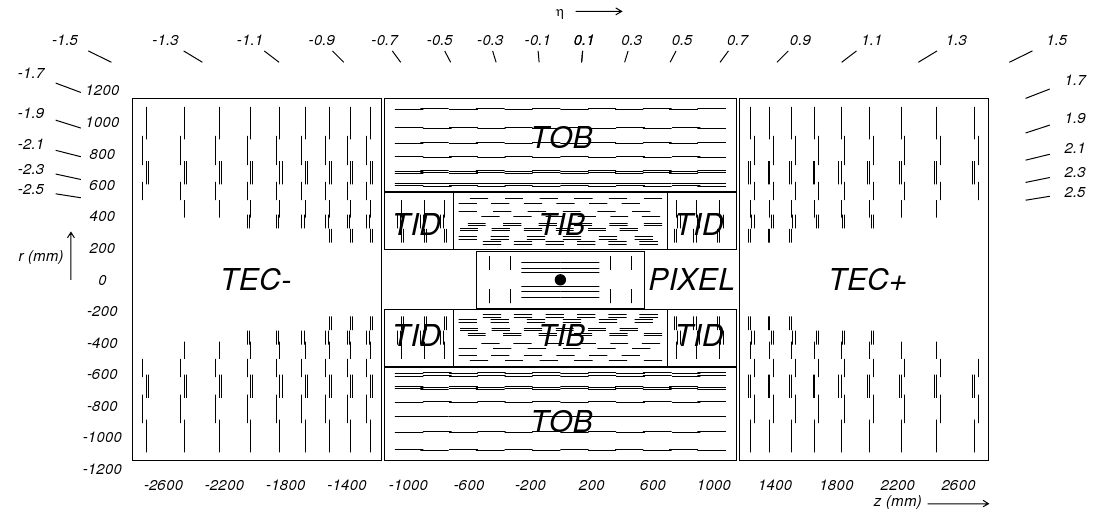
\includegraphics[width=0.7\textwidth]{figures_and_tables/experimental_setup/tracker.png}
    \caption{ Schematic cross section through the CMS tracker. Each line represents a detector
    module. Double lines indicate back-to-back modules which deliver stereo hits. Source:~\cite{Chatrchyan:2008zzk}.}
    \label{cms_tracker}
\end{figure}

The pixel detector consists of 3 layers~\footnote{After 2017, the pixel received one more layer, but this irrelevant to the context of this study, since the data analyzed was collected during 2016.} on the barrel region and 4 layers on the endcap~\footnote{From 2017, another layer on each side was added.}. The pixel is located in a region of 20 cm from the beam pipe.

Each pixel sensor has 100 by 150 $\mu m^2$. The silicon strips detector covers a area of $\approx 200 m^2$ with $9.3 \times 10^6$ channels. It is the largest silicon detector covered area ever built. It is divided in Tracker Inner Barrel (TIB), with length of 130 cm covering the central part of the detector, the Tracker Inner Disks (TID) at the inner endcap, both are surrounded by the Tracker Outer Barrel (TOB) on the barrel, and the Tracker Endcap (TEC).

The tracker is essential for a proper muon measurement in this study.
